% This file was created by tikzplotlib v0.9.8.
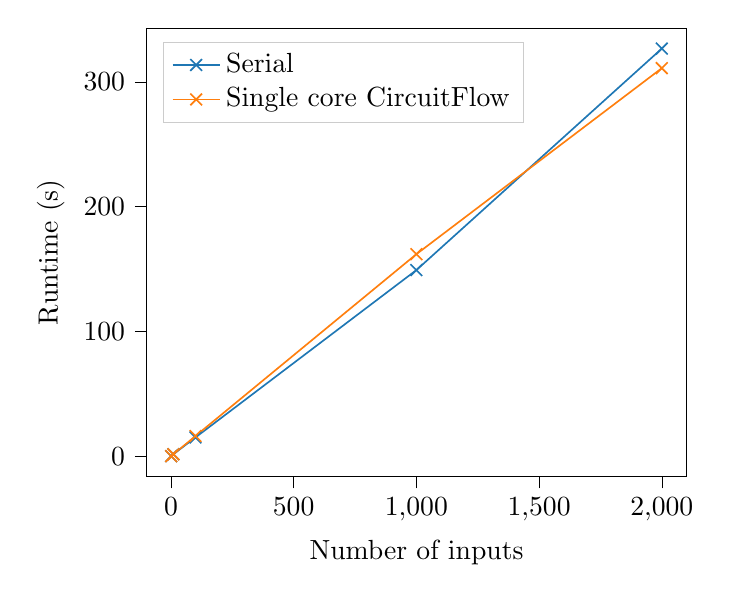
\begin{tikzpicture}

\definecolor{color0}{rgb}{0.12156862745098,0.466666666666667,0.705882352941177}
\definecolor{color1}{rgb}{1,0.498039215686275,0.0549019607843137}

\begin{axis}[
legend cell align={left},
legend style={
  fill opacity=0.8,
  draw opacity=1,
  text opacity=1,
  at={(0.03,0.97)},
  anchor=north west,
  draw=white!80!black
},
tick align=outside,
tick pos=left,
x grid style={white!69.0196078431373!black},
xlabel={Number of inputs},
xmin=-98.95, xmax=2099.95,
xtick style={color=black},
y grid style={white!69.0196078431373!black},
ylabel={Runtime (s)},
ymin=-16.151733195, ymax=342.970146295,
ytick style={color=black}
]
\addplot [semithick, color0, mark=x, mark size=3, mark options={solid}]
table {%
1 0.185249
10 1.7491184
100 15.181053
1000 149.227024
2000 326.6464245
};
\addlegendentry{Serial}
\addplot [semithick, color1, mark=x, mark size=3, mark options={solid}]
table {%
1 0.1719886
10 1.6498082
100 16.326348
1000 161.959576
2000 310.947742
};
\addlegendentry{Single core CircuitFlow}
\end{axis}

\end{tikzpicture}
